\subsection{4.3. 进行中的转移}\label{transitions-in-progress}

本节在四种设定下扩展基础演算。第一种提供第~3.2 节要求、而第~4.2 节无法表达的东西：一次跨越其依赖者可能占据的区间的停用；其余三种则放弃"转移是原子的、即时的、永不出错的"这一理想化——真实运行时中的转移三者皆不具备。被放弃的是"整个转移是一步"这一观念，而不是"一步是对一条规则的一次应用"这一观念。四种设定共享同一个结构性后果，此处一并说明：一个不是一步的转移，在其实施期间需要一个可供占据的状态，且它可能运行的每个方向各有一个状态。

\textbf{定义 49.} 本节的生命周期状态把 \(\Theta _ { \Gamma }\) 替换为

\[
\Theta _ { \Gamma } : = \mathsf { I n a c t i v e } ( \zeta ) \mid \mathsf { R e l o a d i n g } ( i , g , \omega ) \mid \mathsf { A c t i v e } ( g , \omega ) \mid \mathsf { U n l o a d i n g } ( g , \omega , \zeta )\tag{43}
\]

其中 \(i : \mathfrak { E } _ { \Gamma } ^ { \mathrm { i t e r * } }\) 是余下要执行的效应迭代器（见下面的定义~51），\(g : \Gamma \to \Gamma\) 是迄今累积起来的累加器，\(\omega : d \to \mathfrak { N}\) 是已提交视图，\(\zeta : \{ \bot \} \cup \Xi\) 是结果：由 \(\mathsf { U n l o a d i n g }\) 携带的、其停用所指向的那个，以及由 \(\mathsf { I n a c t i v e }\) 携带的、其最终到达的那个——它要么是 \(\bot\)，要么是取自第~4.3.4 节所提供错误集合 \(\Xi\) 的一个错误。

当一个纤维处于携带累加器和已提交视图的三种状态之一时，它被视为已安装（installed）；当它携带错误结果时，则被视为已失败（failed）：

\[
\operatorname { i n s t a l l e d } _ { n } ( \gamma ) : = \theta _ { n } \neq \mathsf { I n a c t i v e } ( - ) , \qquad \operatorname { f a i l e d } _ { n } ( \gamma ) : = \exists \xi \in \Xi . \theta _ { n } = \mathsf { I n a c t i v e } ( \xi )\tag{44}
\]

已安装纤维 \(n\) 在 \(\omega _ { n } ( k ) = m\) 时把键 \(k\) 解析到 \(m\)。定义~46 的静默（quiescence）在这个更宽的状态空间上读作

\[
\mathrm { q u i e t } ( \gamma ) : = \forall n \in \mathrm { d o m } ( F _ { \gamma } ) . \left\{ \begin{array} { l l } { \zeta \neq \bot \vee \mathrm { t a r g e t } _ { n } ( \gamma ) = \bot } & { \mathrm { i f ~ } \theta _ { n } = \mathsf { I n a c t i v e } ( \zeta ) } \\ { \mathrm { t a r g e t } _ { n } ( \gamma ) = \omega _ { n } } & { \mathrm { i f ~ } \theta _ { n } = \mathsf { A c t i v e } ( - , \omega _ { n } ) } \\ { \bot } & { \mathrm { o t h e r w i s e } } \end{array} \right.\tag{45}
\]

第~4.1 节的定义同样适用于这个状态空间，但有两处读法需要确定。第一，第~4.2 节中的 \(\mathsf { I n a c t i v e }\) 在 O-Insert 的结论中读作 \(\mathsf { I n a c t i v e } ( \perp )\)，在 O-Remove 的前提中读作 \(\mathsf { I n a c t i v e } ( - )\)。第二，\(\sigma _ { \gamma }\) 仍只取 \(\mathsf { A c t i v e }\) 纤维之表的并集，因此一个转移正向某个方向进行的纤维，通过它持有的 \(\omega\) 读取自己的余效应，而不提供任何自身的余效应；于是，其转移已经写入的键，还不是依赖者可以据以激活的键。在双状态演算中这一区分是空洞的：那里的每个已安装纤维都是 \(\mathsf { A c t i v e }\)。

图 2 描绘了这些状态形成的生命周期，下面四个小节给出其各边上的规则。

\pandocbounded{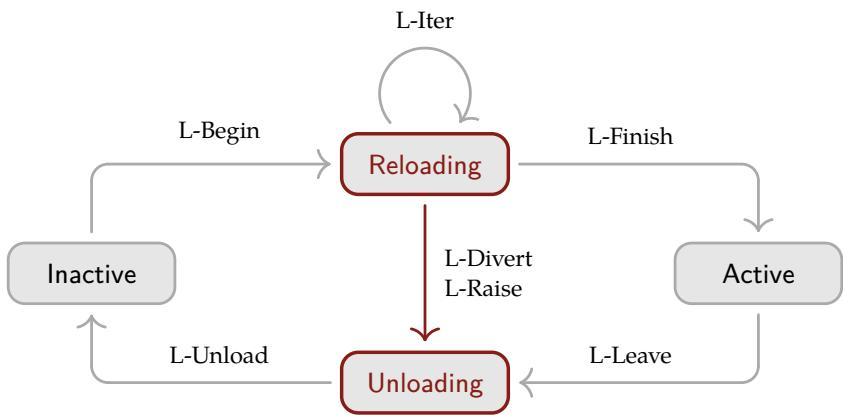
\includegraphics[keepaspectratio,alt={image}]{images/292085ac3f4ef886f94c611c14a57c3de3fd5a92462c7a5892130e190975f400.jpg}}

图 2 \textbar{} 进行中的转移生命周期；两个转移状态以轮廓框出

\subsection{4.3.1. 撤回}\label{withdrawal}

第~3.2 节要求依赖者在它们的依赖之后激活，也要求依赖只在它们的依赖者停用之后撤回其供给。前半句在基础演算中已经成立：激活要求 \(\gamma \models d _ { n }\)，所以声明键 \(k\) 的纤维，在任何纤维活跃地提供 \(k\) 之前都不能激活。后半句才是实质性的，它必须交付的比状态变化的排序更多。一个因其提供者即将离开而被拆除的组件，正在运行它自己的拆除（teardown）代码，而这段代码可能需要正是被撤回的那个余效应；关闭连接池通常意味着把连接交还给提供它们的东西。后半句必须交付的是：消费者在整个停用期间仍能读取 \(k\)，且提供者对 \(k\) 的撤回只有在之后才生效。基础演算根本做不到这一点：其 L-Unload 把撤销供给与运行逆操作放在同一步中执行，在两者之间没有留下可供消费者拆除代码占据的区间。

这一层把这个步骤拆成两步，并用如下条件守卫后半句。

\textbf{定义 50.} 当某个其他已安装纤维把某个键解析到它时，纤维 \(n\) 在 \(\gamma\) 处被依赖（relied upon）：

\[
\begin{array} { r l } & { \mathrm { r e l i e d } _ { n } ( \gamma ) : = \exists m \in \mathrm { d o m } \bigl ( F _ { \gamma } \bigr ) , k \in d _ { m } . m \neq n \land \mathrm { i n s t a l l e d } _ { m } ( \gamma ) \land \omega _ { m } ( k ) = n } \\ & { \qquad \quad \frac { \theta _ { n } = \mathsf { A c t i v e } ( g , \omega ) \quad \mathrm { t a r g e t } _ { n } ( \gamma ) \neq \omega } { \gamma \longrightarrow \gamma [ \theta _ { n } \mapsto \mathsf { U n l o a d i n g } ( g , \omega , \perp ) ] } \quad \mathrm { L \cdot L e a v e } } \\ & { \qquad \quad \frac { \theta _ { n } = \mathsf { U n l o a d i n g } ( g , \omega , \zeta ) \quad \neg \mathrm { r e l i e d } _ { n } ( \gamma ) \quad g ( \gamma ) = \delta } { \gamma \longrightarrow \delta [ \theta _ { n } \mapsto \mathsf { I n a c t i v e } ( \zeta ) ] } \quad \mathrm { L \cdot U n l o a d } } \end{array}\tag{46}
\]

L-Leave 记录停用的决定而不付诸行动，这使纤维停止提供其余效应，同时保持它自己的已提交视图以及其他所有纤维的视图完好。L-Unload 应用累加器、丢弃已提交视图，并让纤维以其携带的结果处于 \(\mathsf { I n a c t i v e }\)；该结果是 \(\bot\)，直到第~4.3.4 节提供另一种情形。它是整个演算中唯一应用累加器的规则。

排序的两个半部随后由该形式的不同部分承担：可见性半部由已提交视图承担，L-Unload 将其丢弃作为最后一个动作；排序半部由前提 \(\neg \mathrm { r e l i e d } _ { n } ( \gamma )\) 承担，我们称之为守卫，它把对 \(k\) 的撤回按捺住，直到每个把 \(k\) 解析到 \(n\) 的消费者都已离开。定理~63 证明了两者。

守卫按绑定而非按纤维施加：\(\mathrm { r e l i e d } _ { n } ( \gamma )\) 检验是否有某个已提交视图点名 \(n\)，因此一个不声明 \(n\) 的任何键的纤维不构成障碍，在另一个域（第~3.2.3 节）中解析过 \(n\) 的某个键的纤维同样不构成障碍。在第~4.2 节的单一来源规约下，按绑定的读法与更粗略的检验 \(\exists m \neq n ,\ k \in d _ { m } .\ \mathrm { i n s t a l l e d } _ { m } ( \gamma ) \wedge k \in p _ { n }\) 一致——在那里，一个键只有一个可能的提供者。

这类守卫通常会死锁。使其免于死锁的是 \(\mathsf { U n l o a d i n g }\) 以及 \(\sigma _ { \gamma }\) 只取 \(\mathsf { A c t i v e }\) 纤维之表的并集：一旦 L-Leave 已标记 \(n\)，其表就离开 \(\sigma _ { \gamma }\)，于是任何目标视图都不能再点名 \(n\)，且每个已向 \(n\) 作出承诺的消费者自己也正在离开。定理~66 把它转化为"守卫总能解除"这一论断。

守卫沿余效应而非沿纤维树为停用排序：父亲可以在它的一个孩子仍处于 \(\mathsf { U n l o a d i n g }\) 时运行其逆操作，因为 relied 只涉及已提交视图。相应地，父亲与孩子之间的排序比定理~63 对提供者与其消费者的排序更弱；而那些效应在环境状态中相遇的父亲与孩子，则由定义~60 的独立性假设支配。

\subsection{4.3.2. 迭代}\label{iteration}

一次激活可以依次执行多个效应，而停用必须把它们全部恢复。我们用效应迭代器（effect iterator）来建模这样的激活：其每一次迭代都产出修改后的上下文、一个逆操作和一个续体（continuation）：

\textbf{定义 51.} 把效应迭代器 \(\mathfrak { E } _ { \Gamma } ^ { \mathrm { i t e r } }\) 和带见证的效应迭代器 \(\mathfrak { E } _ { \Gamma } ^ { \mathrm { i t e r * } }\) 定义为如下递归类型：

\[
\begin{array} { r l } & { \mathfrak { E } _ { \Gamma } ^ { \mathrm { i t e r } } : = \mu \mathfrak { I } . \Gamma \to \Gamma \times ( \Gamma \to \Gamma ) \times \mathsf { M a y b e } ( \mathfrak { I } ) } \\ & { \mathfrak { E } _ { \Gamma } ^ { \mathrm { i t e r * } } : = \mu \mathfrak { I } . \left( e : \Gamma \to \Gamma \times ( \Gamma \to \Gamma ) \times \mathsf { M a y b e } ( \mathfrak { I } ) \right) } \\ & { \qquad \times \left( ( \gamma : \Gamma ) \to ( \mathbf { l e t } \ ( \delta , g , o ) = e ( \gamma ) \ \mathbf { i n } \ g ( \delta ) \simeq \gamma ) \right) } \end{array}\tag{47}
\]

其中 \(e ( \gamma )\) 产出三元组 \(( \delta , g , o )\)，分别表示：

• \(\delta\) 是新上下文；

• \(g\) 是当前效应的逆函数；

• \(o\) 指示续体：

‣ \(\mathsf { N o t h i n g }\) 表示迭代终止；

‣ \(\mathsf { J u s t } ( i )\) 提供下一次迭代。

见证按定义~33 的 ≃ 来读，正如定义~37 读 \(\mathfrak { E } _ { \Gamma } ^ { * }\) 的见证那样：当 \(i\) 尊重 ≃ 且其产出的每个 \(g\) 都尊重 ≃ 并满足上面那条子句时，\(i \in \mathfrak { E } _ { \Gamma } ^ { \mathrm { i t e r } }\) 属于 \(\mathfrak { E } _ { \Gamma } ^ { \mathrm { i t e r * } }\)。三元组按分量比较：\(\mathsf { N o t h i n g }\) 只与 \(\mathsf { N o t h i n g }\) 比较，\(\mathsf { J u s t } ( i )\) 与 \(\mathsf { J u s t } ( i ^ { \prime } )\) 比较需当 \(i \simeq i ^ { \prime }\)；迭代器上的 ≃ 是满足这些子句的最大关系。把 ≃ 取为 \(\Gamma\) 上的相等，即恰好恢复该读法。

效应迭代器变换 \(\mathrm { e f f e c t } _ { \Gamma } ^ { \mathrm { i t e r } }\) 通过递归调用把 \(\mathrm { e f f e c t } _ { \Gamma }\) 扩展到迭代器结构上：

\textbf{定义 52.} 把效应迭代器变换 \(\mathrm { e f f e c t } _ { \Gamma } ^ { \mathrm { i t e r } }\) 定义为：

\[
\begin{array} { r l } & { \mathrm { e f f e c t } _ { \Gamma } ^ { \mathrm { i t e r } } : \mathfrak { E } _ { \Gamma } ^ { \mathrm { i t e r } } \to \partial \Gamma \to \partial ^ { 2 } \Gamma } \\ & { \mathrm { e f f e c t } _ { \Gamma } ^ { \mathrm { i t e r } } = i \mapsto ( \gamma , \varphi ) \mapsto \mathbf { l e t } \ ( \delta , g , o ) = i ( \gamma ) \ \mathbf { i n } \ \mathbf { l e t } \ t = \mathrm { t r a c k } _ { \Gamma } ( g , \mathrm { p r } _ { 1 } \circ i ) \ \mathbf { i n } \ \mathbf { m a t c h } \ o } \\ & { \qquad \quad | \ \mathsf { N o t h i n g } \Rightarrow ( ( \delta , \varphi \circ g ) , t ) } \\ & { \qquad \quad | \ \mathsf { J u s t } ( i ^ { \prime } ) \Rightarrow \mathbf { l e t } \ ( s , r ) = \mathrm { e f f e c t } _ { \Gamma } ^ { \mathrm { i t e r } } ( i ^ { \prime } ) ( \delta , \varphi \circ g ) \ \mathbf { i n } \ ( s , t \circ r ) } \end{array}\tag{48}
\]

在每一次迭代中，逆操作 \(g\) 按应用顺序复合到 \(\varphi\) 上，因此累加器 \(\varphi \circ g _ { 1 } \circ \cdots \circ g _ { k }\) 在应用时自然地按后进先出（LIFO）顺序恢复效应。因为 \(\mathrm { e f f e c t } _ { \Gamma } ^ { \mathrm { i t e r } }\) 落在与 \(\mathrm { e f f e c t } _ { \Gamma }\) 相同的 \(\partial \Gamma \to \partial ^ { 2 } \Gamma\) 中，迭代器本身就是一种效应，可以在任何效应可用的地方使用。组件的整个激活就是这样一个用途——这正是本节其余部分要形式化的内容——并且实现允许在每个变更点（mutation site）接受迭代器（第~5.1.1 节）。\(\mathsf { M a y b e } ( \mathfrak { E } ^ { \mathrm { i t e r } } )\) 续体在任何两次相邻迭代之间提供了边界：在该边界处，上下文就是迄今各次迭代所形成的上下文，而累加器恢复的也正是这些迭代所产生的东西，不多不少。在这个意义上，效应迭代器是一种具象化的定界续体（delimited continuation）——主流语言通过 yield 运算符暴露的那种结构 {[}43{]}——因此该模型直接对接到它们已经提供的生成器（generator）上。

在演算中，从此刻起，定义~44 的 \(e _ { n }\) 按 \(\mathfrak { E } _ { \Gamma } ^ { \mathrm { i t e r * } }\) 来读；把原子效应函数替换为迭代器，把基础 L-Reload 拆成一个迹线（trace）所经过的"已开始"状态，并给纤维一个离开该状态的第二条出路。

\[
\begin{array} { r l } & { \frac { \theta _ { n } = \mathsf { I n a c t i v e } ( \perp ) \quad \omega = \mathrm { t a r g e t } _ { n } ( \gamma ) \neq \perp } { \gamma \longrightarrow \gamma [ \theta _ { n } \mapsto \mathsf { R e l o a d i n g } ( e _ { n } , \mathrm { i d } _ { \Gamma } , \omega ) ] } \quad \mathrm { L \cdot B e g i n } } \\ & { \frac { \theta _ { n } = \mathsf { R e l o a d i n g } ( i , g , \omega ) \quad \mathrm { t a r g e t } _ { n } ( \gamma ) \neq \omega \quad ( \delta , h ) = ( \gamma , \mathrm { i d } _ { \Gamma } ) \vee i ( \gamma ) = ( \delta , h , - ) } { \gamma \longrightarrow \delta [ \theta _ { n } \mapsto \mathsf { U n l o a d i n g } ( g \circ h , \omega , \perp ) ] } \quad \mathrm { L \cdot D i v e r t } } \\ & { \frac { \theta _ { n } = \mathsf { R e l o a d i n g } ( i , g , \omega ) \quad \mathrm { t a r g e t } _ { n } ( \gamma ) = \omega \quad i ( \gamma ) = ( \delta , h , \mathsf { J u s t } ( i ^ { \prime } ) ) } { \gamma \longrightarrow \delta [ \theta _ { n } \mapsto \mathsf { R e l o a d i n g } ( i ^ { \prime } , g \circ h , \omega ) ] } \quad \mathrm { L \cdot I t e r } } \\ & { \frac { \theta _ { n } = \mathsf { R e l o a d i n g } ( i , g , \omega ) \quad \mathrm { t a r g e t } _ { n } ( \gamma ) = \omega \quad i ( \gamma ) = ( \delta , h , \mathsf { N o t h i n g } ) } { \gamma \longrightarrow \delta [ \theta _ { n } \mapsto \mathsf { A c t i v e } ( g \circ h , \omega ) ] } \quad \mathrm { L \cdot F i n i s h } } \end{array}
\]

每次迭代都按定义~52 把新产出的逆操作以 \({ \boldsymbol { g } } \circ { \boldsymbol { h } } ,\) 复合到累加器上，因此累加器按后进先出顺序应用这些逆操作。在任意两次相邻迭代之间，如果目标视图已变化，系统可以转移（divert）该转移，并应用迄今累积的逆操作来恢复上下文。与所有其他停用一样，L-Divert 经由 \(\mathsf { U n l o a d i n g }\) 走，而不是就地应用累加器；它在那里遇到的守卫是空的——一个从未处于 \(\mathsf { A c t i v e }\) 的纤维不提供任何东西，也不出现在任何已提交视图中。它的两个分支中的第一个中止纤维所持有的迭代——只有迭代边界才能使这成为可能，因此转移可以落下的粒度就是迭代器的粒度；第二个分支让该迭代落地，而第~4.3.3 节正是需要它的地方。

普通的效应函数 \(( \mathfrak { E } _ { \Gamma } )\) 是退化情形，其中第一次迭代就已产出 \(\mathsf { N o t h i n g }\)。这样的转移仍经过 \(\mathsf { R e l o a d i n g }\)，L-Divert 在那里仍然适用，但累加器是 \(\mathrm { i d } _ { \Gamma }\)，且没有任何迭代运行过，因此什么都不会被恢复，转移要么安装其全部效应，要么一个都不安装。

\subsection{4.3.3. 异步}\label{asynchrony}

迄今为止的各层允许环境在两次相邻迭代之间移动，并假定每次迭代本身瞬时完成，其发起与落地是一步。我们抽象地建模这种非即时性：一次迭代产出一个类型为 \(\mathsf { F u t u r e } ( A )\) 的值，其中 \(\mathsf { F u t u r e }\) 是一个不透明的类型构造子，其定义性性质是：在提交（submission）与完成（resolution）之间，外部状态可能改变。

在这个模型下，一次迭代在一个状态发起、在另一个状态落地，纤维在飞行期间处于 \(\mathsf { R e l o a d i n g }\)。这一层添加的是惯性：一旦发起，迭代就会落地，且其落地不能被拒绝。因此，在飞行期间转向的目标视图不能通过中止迭代来回应，只剩下 L-Divert 中让迭代落地的那一分支可用：迭代落地，随后纤维停用。所以这一层不添加任何规则，也不添加任何规则所匹配的类型；在 \(\Gamma\) 的粒度上，惯性就是它的全部内容，其形式是对宿主可以采取 L-Divert 的哪个分支的限制。

那个分支正是基础演算无法表达的东西。在那里，目标视图已转向的转移在发现它的同一步中被撤销；在这里，飞行中的迭代必须先落地，所以纤维在逆操作运行期间需要一个去处，唯一可靠的地方是持有该迭代所产出逆操作的 \(\mathsf { U n l o a d i n g }\)。改走 \(\mathsf { A c t i v e }\) 会让纤维在一步的长度内提供其余效应，并迫使它的依赖者去针对一个已经离开的组件激活。这就是实现中 reload 与 unload 的相互链接。

停用也可以直接链接回激活——通过复合（composite）而非规则。L-Unload 对目标视图不携带任何前提，因此无论纤维停用期间目标视图变成了什么，累加器都会运行，纤维变为 \(\mathsf { I n a c t i v e }\)，而 L-Begin 可以从该状态立即开始一次新的转移。

\subsection{4.3.4. 失败}\label{failure}

迄今的每条规则都假定它所运行的效应成功，而运行时做不到。组件安装的效应延伸到了跟踪它们的上下文之外，它们触及的东西可能拒绝：一个已绑定的端口、一个不存在的文件、一个不应答的对端。失败的转移仍必须让纤维的效应得到恢复，而不是搁浅。

令 \(\Xi\) 是一个错误集合，并精化定义~51 的效应迭代器，使迭代可以抛错（raise）而不产出三元组：

\[
\begin{array} { r l } & { \mathfrak { E } _ { \Gamma } ^ { \mathrm { f a i l } } : = \mu \mathfrak { I } . \Gamma \to \mathsf { E i t h e r } ( \Xi , \Gamma \times ( \Gamma \to \Gamma ) \times \mathsf { M a y b e } ( \mathfrak { I } ) ) } \\ & { \mathfrak { E } _ { \Gamma } ^ { \mathrm { f a i l } * } : = \mu \mathfrak { I } . \left( e : \Gamma \to \mathsf { E i t h e r } ( \Xi , \Gamma \times ( \Gamma \to \Gamma ) \times \mathsf { M a y b e } ( \mathfrak { I } ) ) \right) } \\ & { \qquad \times \left( ( \gamma : \Gamma ) \to ( \mathbf { l e t } \ \mathsf { R i g h t } ( \delta , g , o ) = e ( \gamma ) \ \mathbf { i n } \ g ( \delta ) \simeq \gamma ) \right) } \end{array}\tag{49}
\]

见证只约束 \(\mathsf { R i g h t }\) 这一情形，在模式不匹配处是空条件——一次抛错没有可撤销的东西；从此刻起，\(\mathsf { R e l o a d i n g }\) 携带的 \(i\) 按 \(\mathfrak { E } _ { \Gamma } ^ { \mathrm { f a i l } * }\) 来读。定义~52 的提升（lift）也照搬过来，只是把抛错替代三元组进行传播，因此正如普通迭代器一样，会抛错的迭代器可以在任何效应可用的地方使用。这一层添加一条规则，并把定义~49 的第二种结果投入使用，O-Remove 无需加宽即可接纳它。L-Iter、L-Finish 和 L-Divert 的前提中，它们所匹配的三元组外层都读作 \(\mathsf { R i g h t }\)。抛错是迭代所做的事情，因此这条规则是从 \(\mathsf { R e l o a d i n g }\) 退出。

\[
\frac { \theta _ { n } = \mathsf { R e l o a d i n g } ( i , g , \omega ) \quad i ( \gamma ) = \mathsf { L e f t } ( \xi ) } { \gamma \longrightarrow \gamma [ \theta _ { n } \mapsto \mathsf { U n l o a d i n g } ( g , \omega , \xi ) ] } \quad \mathrm { L \cdot R a i s e }
\]

L-Raise 先恢复后记录。纤维带着作为其结果的错误进入 \(\mathsf { U n l o a d i n g }\)，在那里应用累积到失败迭代为止的累加器，随后纤维到达 \(\mathsf { I n a c t i v e } ( \xi )\)，什么也没有安装；这个状态与中止式 L-Divert 本会产生的状态相比，只在纤维所携带的结果上不同。像所有其他停用一样处理失败，正是使每个结果只能通过 L-Unload 到达的原因，这也是定理~59 所依据的单一事实。L-Begin 以 \(\mathsf { I n a c t i v e } ( \perp )\) 为前提，因此生命周期不会从错误结果重新进入；这就是结果的实质——它扣住一个其效应函数在其运行所针对的状态中已被证明不可靠的纤维，而不是在不变的环境中对它重试。失败的纤维也不阻碍任何东西：它是 \(\mathsf { I n a c t i v e }\)，因此不携带已提交视图，也无法使 relied 成立。

失败记录在纤维上，而不是传播给其父亲，因此转移失败的组件会留下其兄弟继续运行——这正是插件宿主想要的行为，也是结果按纤维记录、而非作为整个状态属性的原因。
